%!TEX root = paper.tex
%related.tex

\section{Related work}
\label{sec:related}

\subsection{Imbalances of Power}
This work falls within a line of research that investigates imbalances of power between citizens and institutions, such as governments or corporations. In~\cite{laskowskigovernment}, we investigated the issue of government surveillance.  Our main takeaway was that increased surveillance technology increases incentives for abuse. In  \cite{johnsoncaviar}, we considered the welfare of consumers as a result of corporate exchanges of personal data.
We found that when consumers are myopic, firms benefit greatly, but consumer surplus is also reduced. When we assume that consumers are strategic, a more complex picture emerges. Consumers are better off in this case, but firms fare worse.  Given that firms actually do in fact share consumer data in ways quite similar to our model, consumers cannot be acting strategically.  One might wonder, if a market for consumer data only exists when consumers are non-strategic, is the market exploiting consumers?  Our current work follows this line of investigation on power imbalances by considering the plight of minority groups targeted by unjust laws.

\subsection{Polarization}
Most voters in the United States have been and remain overwhelmingly moderate in their policy positions\cite{layman2006party}. Nevertheless, the United States Congress has passed a number of divisive laws, many of which have been challenged and overturned by the US Supreme Court.  Even in European countries, laws have been passed %xamples in European countries such as France, Belgium, and the Netherlands include laws passed 
against face covering, pejoratively dubbed ``burka bans.''

\begin{figure}[htbp]
\begin{center}
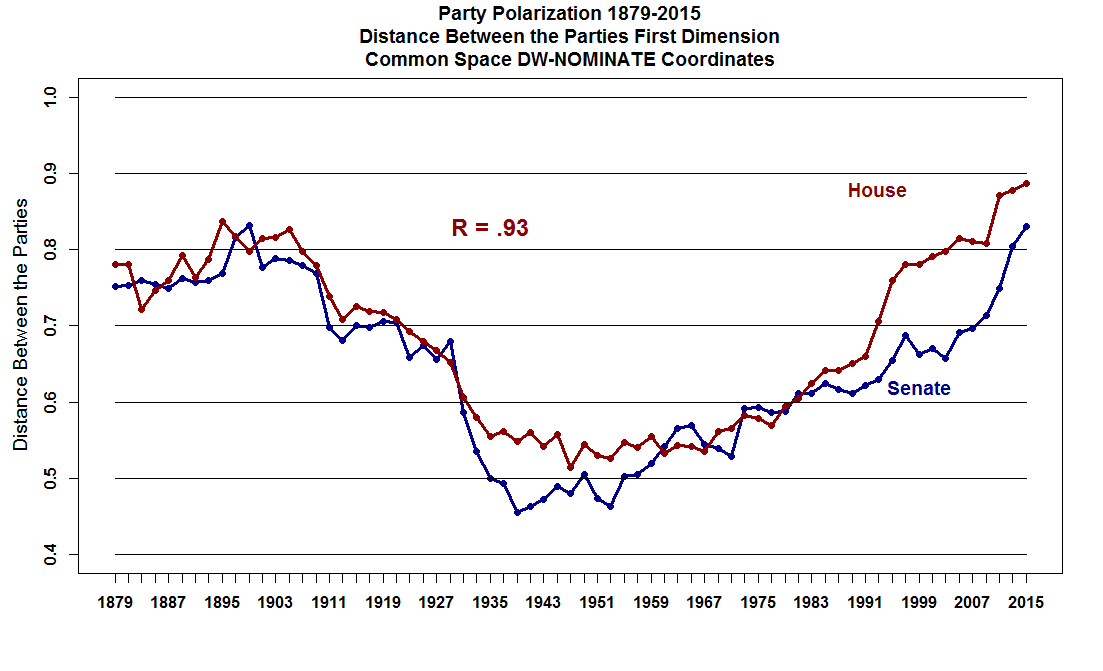
\includegraphics[width=0.4\textwidth]{figs/polar_house_and_senate_46-115_july_11}
\caption{{\bf Polarization Trends in the US Congress}}
\label{fig:uscongress}
\end{center}
\end{figure}

The United States congress in particular has become increasingly polarized over the last 40 years (see Figure \ref{fig:uscongress}); and
researchers have posited a number of reasons for this phenomenon \cite{barber2015causes}\cite{poole1984polarization}, ranging from a polarized electorate, to southern realignment, to gerrymandering, to the evolution of modern primary elections, to economic inequality, to money in politics, to the media environment, or to congress-based factors such as congressional rule changes, majority party agenda control, party pressures, teamsmanship, or the breakdown of bipartisan norms.  All of these issues are discussed in~\cite{poole1984polarization}.
More culturally-specific theories involving authoritarianism are also prevalent \cite{hetherington2009authoritarianism}; and there is a remarkably close correlation between economic
inequality and polarization in the United States~\cite{mccarty2006polarized}.  See Figure \ref{fig:inequality}.

\begin{figure}[htbp]
\begin{center}
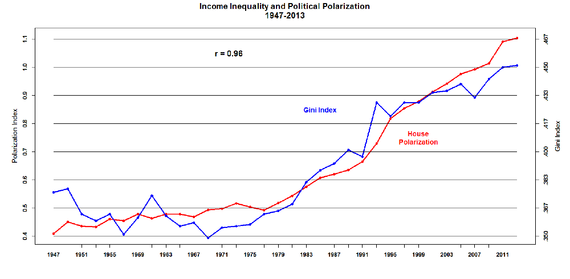
\includegraphics[width=0.4\textwidth]{figs/8141eb7a0}
\caption{{\bf Polarization versus Income Inequality}}
\label{fig:inequality}
\end{center}
\end{figure}


A more economically-driven explanation derives from the notion of information cascades. An information cascade occurs when people receive a noisy signal and rely on friends and colleagues to distill the essential parts.  According to \cite{bikhchandani1992theory},
``An information cascade occurs when it is optimal for an individual, having observed the actions of those ahead of him, to follow the behavior of the preceding individual without regard to his own information." 

The notion that people exhibit herding behavior in predictable circumstances has been around for decades \cite{shiller1995conversation}.  For example, researchers at Iowa State University conducted 259 interviews with farmers who had largely refused offers to adopt drought-resistant seed corn during the Great Depression and Dust Bowl.  They found that the slow rate of adoption was due to ``how farmers valued the opinion of their friends and neighbors instead of the word of a salesman''\cite{beal1957diffusion}.



We include this notion of influenced behavior in our model as a way to explain the source of divisiveness.  Our model does not mandate any herd behavior, but merely allows it.  This allowance appears justified by the observation that the United States has a legislative system that is organized like Figure \ref{fig:partisonship}, while it has an electorate that is more like Figure \ref{fig:voters}.


\begin{figure}[htbp]
\begin{center}
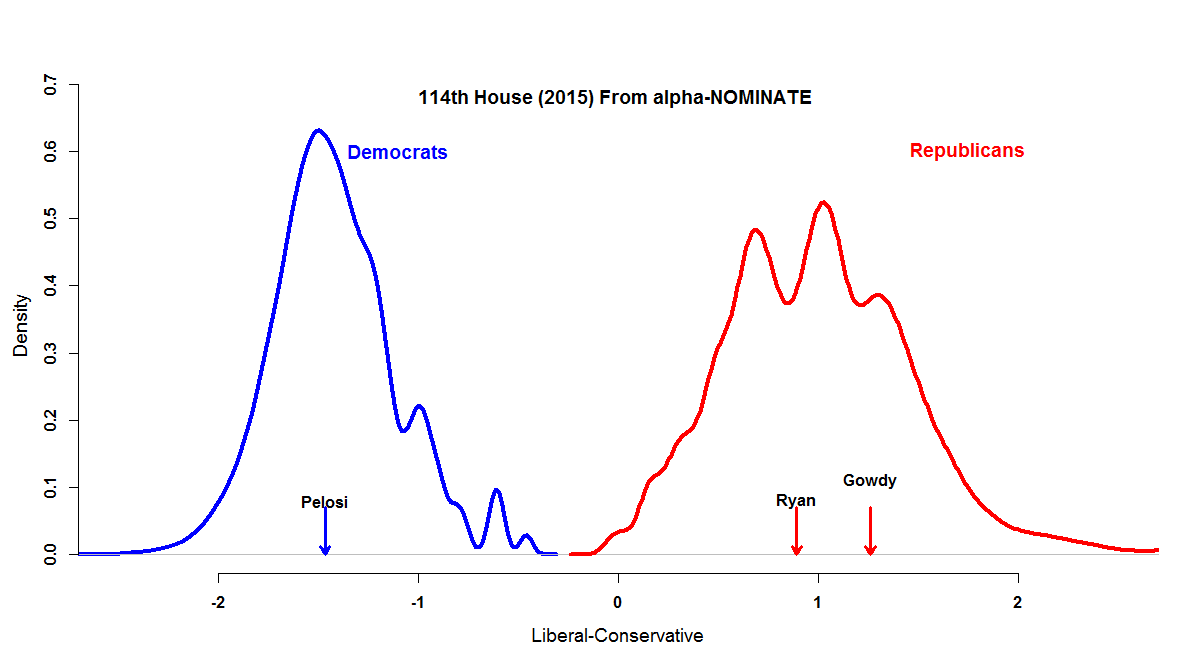
\includegraphics[width=0.4\textwidth]{figs/alpha_House_114_Histogram_8_January_2016}
\caption{{\bf Partisonship in the US House of Representatives}}
\label{fig:partisonship}
\end{center}
\end{figure}




\begin{figure}[htbp]
\begin{center}
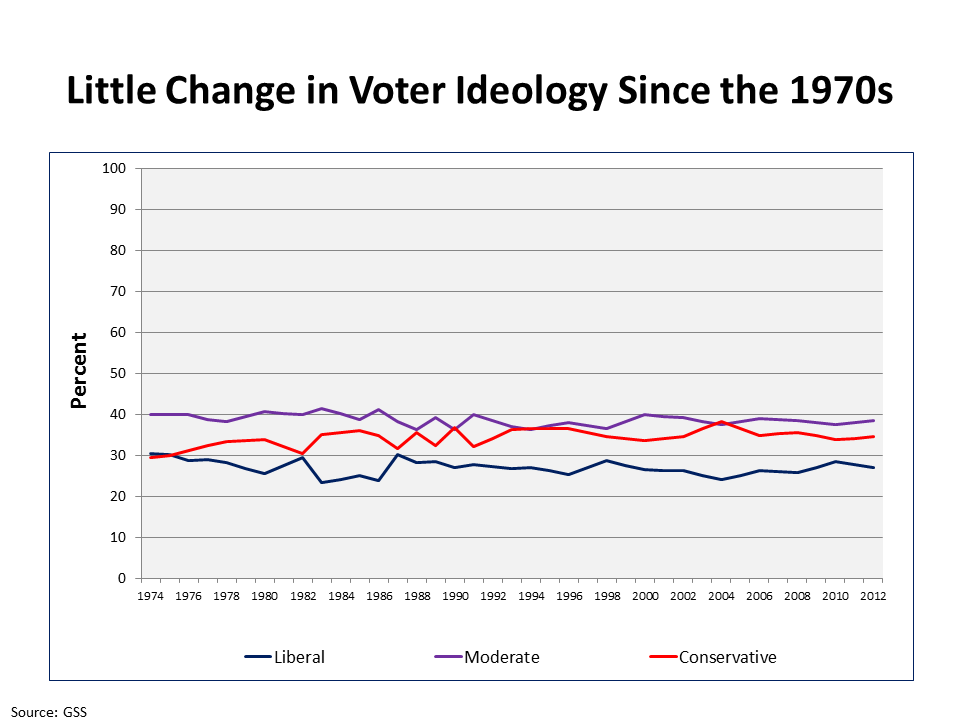
\includegraphics[width=0.4\textwidth]{figs/polarization2}
\caption{{\bf Long Term Trends in US Voter Ideology}}
\label{fig:voters}
\end{center}
\end{figure}


\subsection{Privacy}

Privacy on the ground.



